\newpage
\section{Example Usage}
\paragraph{}Check out \texttt{example.tex} for the contents of this section. This section will be commented out after a while.
\paragraph{}Here is a reference \cite{example2024}. An inline equation $x^2+1=0$, or in display form:
\[\int_0^1 f(x)\mathrm{d}x\]
see also the \texttt{equation, multline, align} environments from the \texttt{amsmath} package.
\paragraph{}A picture can be included using \texttt{includegraphics} (on Overleaf, one may simply use the snippet for begin figure), and referenced via \texttt{ref}, such as \ref{fig:example}; see the top of this page for the graphics included.
\begin{center}
\begin{figure}
    \centering
    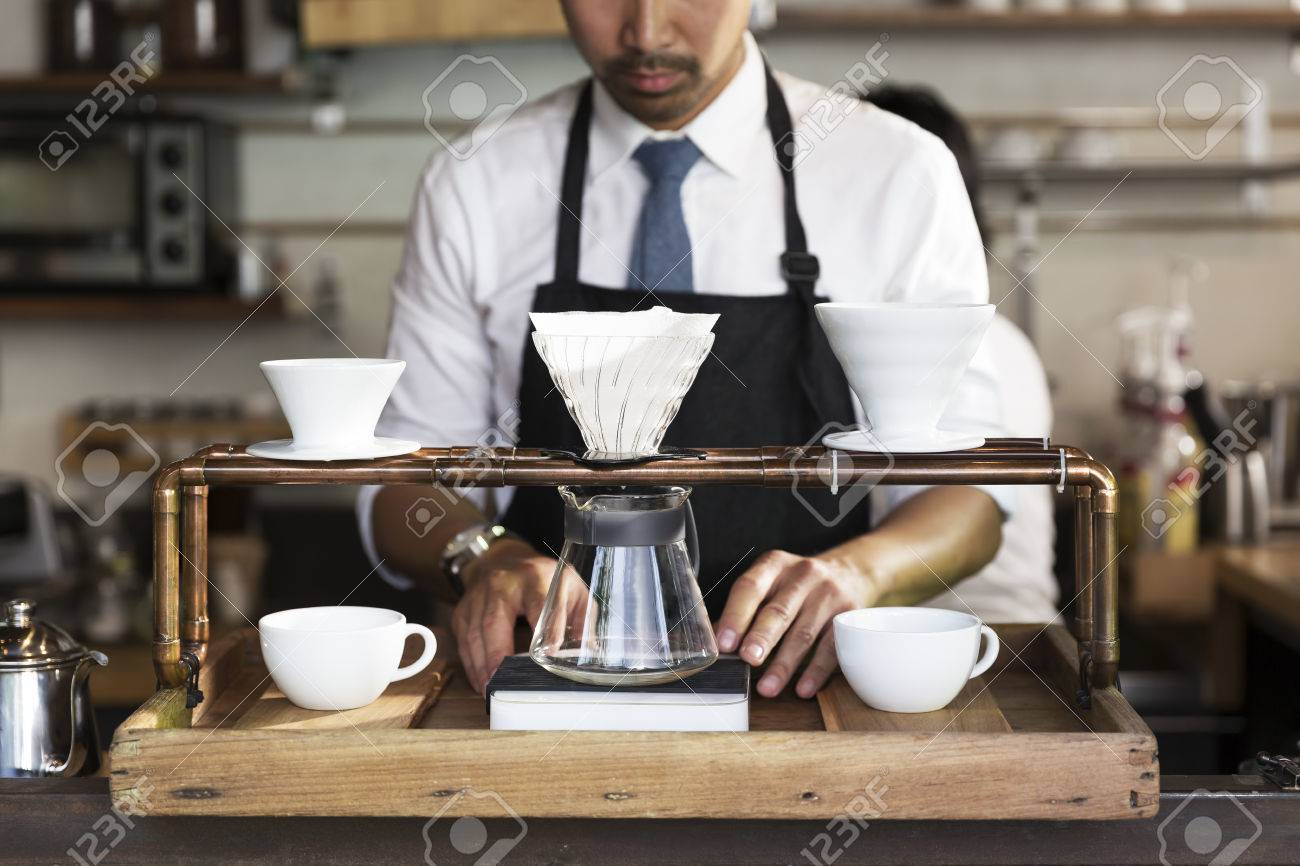
\includegraphics[scale=1]{media/coffee.jpg}
    \caption{a stock photo of coffee making}
    \label{fig:example}
\end{figure}
\end{center}
\paragraph{}Ordered lists and unordered list can be given via the \texttt{enumerate, itemize} environments. For example, the Heilmeier questions:
\begin{enumerate}[label=(\arabic*)]
    \item What are you trying to do? Articulate your objectives using absolutely no jargon.
    \item How is it done today; what are the limits of current practice?
    \item What's new in your approach? Why will it be successful?
    Who cares?
    \item If you're successful, what difference and impact will it make, and how do you measure them (e.g., via user studies, experiments, ground truth data, etc.)?
    \item What are the risks and payoffs?
    \item How much will it cost?
    \item How long will it take?
    \item What are the midterm and final "exams" to check for success? How will progress be measured?
\end{enumerate}
\paragraph{}In short, \texttt{enumerate, itemize, item} are kinda like \texttt{ol, ul, li} in HTML. Appearance of the items can be tuned via packages, such as \texttt{enumitems}.
\paragraph{}One can also add todo via the \texttt{todo} package. For example: \todo{Finish adding contents to this example.}
\paragraph{}One can add URLs like \url{https://www.youtube.com/watch?v=dQw4w9WgXcQ}.
